\vspace{-2mm}
\section{Introduction}
\label{sec:intro}
\vspace{-1mm}

Modern deep learning often trains millions or even billions of parameters~\citep{Devlin:2018bert,shoeybi2019megatron,raffel2019exploring,brown2020language} to deliver good performance for a model. 
Recently, \citet{frankle2018lottery,frankle2020linear} demonstrated that these over-parameterized  networks contain sparse subnetworks, when trained in isolation, that can achieve similar or better performance than the original~model.

Furthermore, recent studies revisit the initialization stage of finding these subnetworks in vision models~\citep{Zhou:2019deconstructing,Ramanujan:2020hidden}.
Such a mask, which is used to mask out a part of the entire network to those subnetworks, is referred to as a ``Supermask.'' 
That is to say, subnetworks of a \textit{randomly weighted neural network} (NN) can achieve competitive performance, which may act as a good  ``prior''~\citep{gaier2019weight} and connect to the long history of leveraging random features~\citep{Gamba:1961papa,Baum:1988jc} and/or random kernel methods~\citep{Rahimi:2008random,Rahimi:2009kitchen} in machine learning. 
Here, we examine the following question: how does a fully randomized natural language processing (NLP) model perform in the multi-layer setting, and particularly in the (so far under-explored) one-layer setting?

\begin{figure}
    \centering
    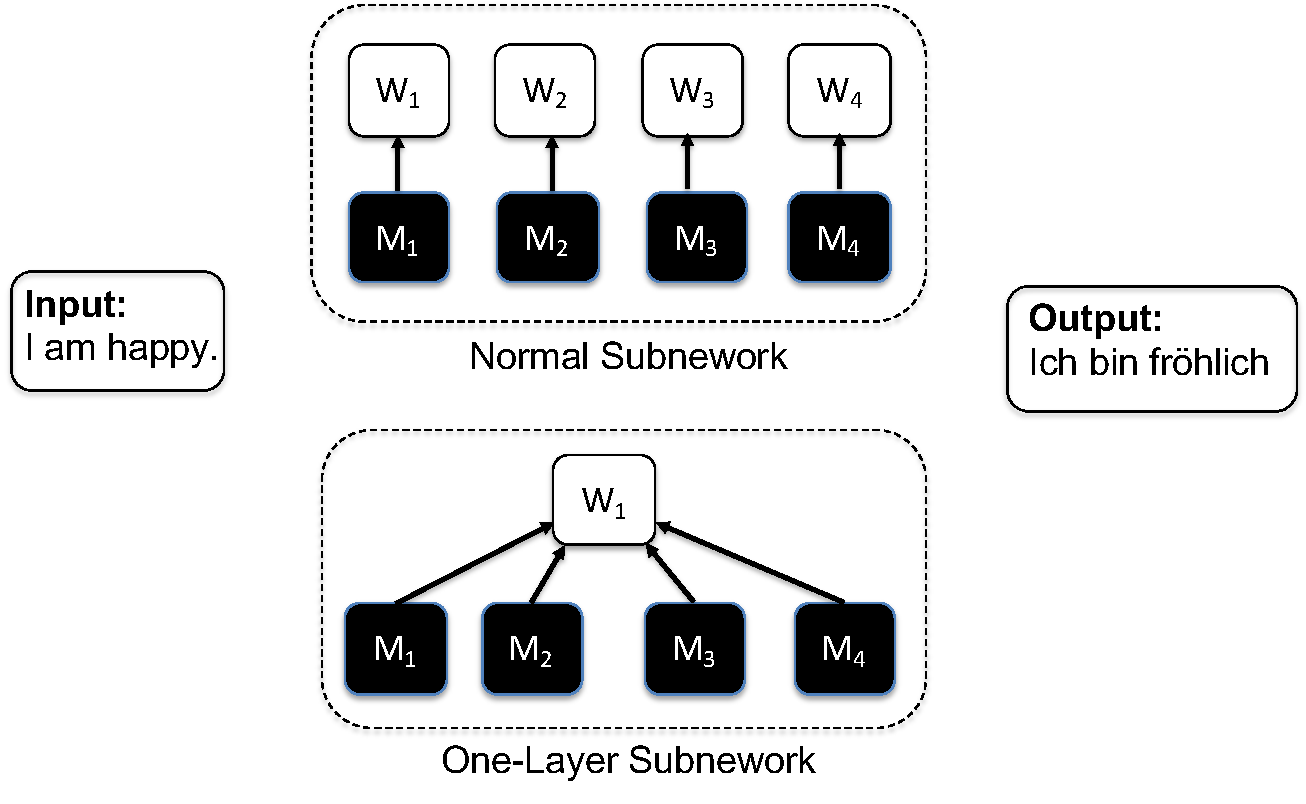
\includegraphics[width=0.8\linewidth]{fig/sketch.pdf}
            \vspace{-5pt}
    \caption{ Illustration plot for a normal subnetwork and a one-layer subnetwork.}
    \label{fig:model_illustration}
    \vspace{-6mm}
\end{figure}

In this work, we first validate that there exist subnetworks of standard randomly weighted Transformers (Reservoir Transformers in~\citep{shen2020reservoir}) that can perform competitively with fully-weighted alternatives on machine translation and natural language understanding tasks. 
With 50\% randomized weights remaining, we found a subnetwork that can reach 29.45/17.29 BLEU on IWSLT14/WMT14, respectively. 
We also investigate the special case of finding subnetworks in one-layer randomly weighted Transformers (see~\fref{fig:model_illustration}). 
To obtain the subnetworks, we repeatedly apply the same randomized Transformer layer several times with different Supermasks. 
The resulting subnetwork of a one-layer randomly-weighted Transformer has similar performance as the multi-layer counterparts with a 30\% lower memory footprint. 
We also study the impact of different depths/widths of Transformers along with the effectiveness of two initialization methods. 
Finally, using the pre-trained embedding layers, we find that the subnetworks hidden in one layer randomly weighted Transformer$_\text{wide/wider}$ are smaller than, but can match 98\%/92\% of the performance of, a trained Transformer$_\text{small/base}$ on IWSLT14/WMT14. 
We hope our findings can offer new insights for understanding Transformers. 